\subsection{UC14 - Posizionamento prodotto in scaffalatura}
\begin{figure}[H]
  \centering
  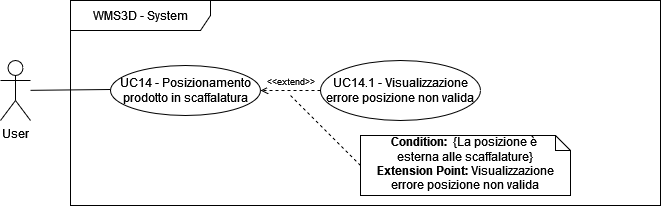
\includegraphics[width=0.8\textwidth]{UC_diagrams_11-20/UC14_sys.drawio.png}
   \caption{Diagramma UML UC14 - Posizionamento prodotto in scaffalatura}
\end{figure}
\begin{figure}[H]
  \centering
  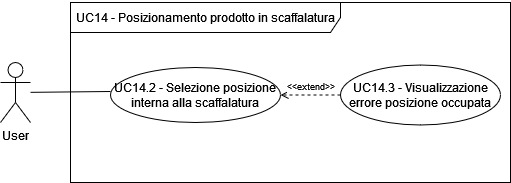
\includegraphics[width=0.8\textwidth]{UC_diagrams_11-20/UC14.drawio.png}
   \caption{Diagramma UML in dettaglio UC14 - Posizionamento prodotto in scaffalatura}
\end{figure}
\begin{itemize}
    \item \textbf{Attori:} User.
    \item \textbf{Pre-condizione:}  L'utente ha creato [UC6] e posizionato [UC7] una scaffalatura e ha creato anche un prodotto [UC13].
    \item \textbf{Post-condizione:} Il prodotto creato è posizionato nella scaffalatura creata presente all'interno del render 3D.
    \item \textbf{Scenario Principale:} L'utente dopo aver creato un prodotto sceglie in quale scaffalatura interna al magazzino posizionare il prodotto, e più specificatamente anche in quale bin interno posizionarlo [UC14.2].
    \item \textbf{Generalizzazioni:} -
    \item \textbf{Estensioni:} È presente una estensione nel caso in cui la posizione non sia valida:
    \begin{itemize}
        \item UC14.1 - Visualizzazione errore posizione non valida.
    \end{itemize}
\end{itemize}


\subsubsection{UC14.1 - Visualizzazione errore posizione non valida}
\begin{itemize}
    \item \textbf{Attori:} User.
    \item \textbf{Pre-condizione:}  L'utente cerca di posizionare il prodotto al di fuori delle scaffalature.
    \item \textbf{Post-condizione:} L'utente visualizza un messaggio d'errore e il posizionamento non viene permesso.
    \item \textbf{Scenario Principale:} L'utente visualizza un messaggio informativo sull'errore. L'utente dovrà cambiare posizionamento.
    \item \textbf{Generalizzazioni:} -
    \item \textbf{Estensioni:} -
\end{itemize}


\subsubsection{UC14.2 - Selezione posizione interna alla scaffalatura}
\begin{itemize}
    \item \textbf{Attori:} User.
    \item \textbf{Pre-condizione:}  L'utente ha creato [UC6] e posizionato [UC7] una scaffalatura e ha creato anche un prodotto [UC13]. 
    \item \textbf{Post-condizione:} Il prodotto creato è posizionato nel bin selezionato nella scaffalatura creata presente all'interno del render 3D.
    \item \textbf{Scenario Principale:} L'utente dopo aver creato un prodotto sceglie in quale bin e di quale scaffalatura posizionare il prodotto.
    \item \textbf{Generalizzazioni:} -
    \item \textbf{Estensioni:} È presente una estensione nel caso in cui il bin scelto sia occupato:
    \begin{itemize}
        \item UC14.3- Visualizzazione errore posizione occupata.
    \end{itemize}
\end{itemize}


\subsubsection{UC14.3 - Visualizzazione errore posizione occupata}
\begin{itemize}
    \item \textbf{Attori:} User.
    \item \textbf{Pre-condizione:}  L'utente cerca di posizionare il prodotto in un bin già occupato da un altro prodotto.
    \item \textbf{Post-condizione:} L'utente visualizza un messaggio d'errore e il posizionamento non viene permesso.
    \item \textbf{Scenario Principale:} L'utente visualizza un messaggio informativo sull'errore. L'utente dovrà cambiare posizionamento.
    \item \textbf{Generalizzazioni:} -
    \item \textbf{Estensioni:} -
\end{itemize}